\documentclass{standalone}
\usepackage{pgfplots}
\usetikzlibrary{colorbrewer}
\usepgfplotslibrary{groupplots}
\pgfplotsset{compat=1.3}

\definecolor{arr2flatcolour}{RGB}{31,120,180}
\definecolor{arr2minncolour}{RGB}{227,26,28}
\definecolor{arr2bumpcolour}{RGB}{51,160,44}
\definecolor{minnesotacolour}{RGB}{255,127,0}
\definecolor{rhscolour}{RGB}{177,89,40}
\definecolor{gaussiancolour}{RGB}{106,61,154}

\begin{document}
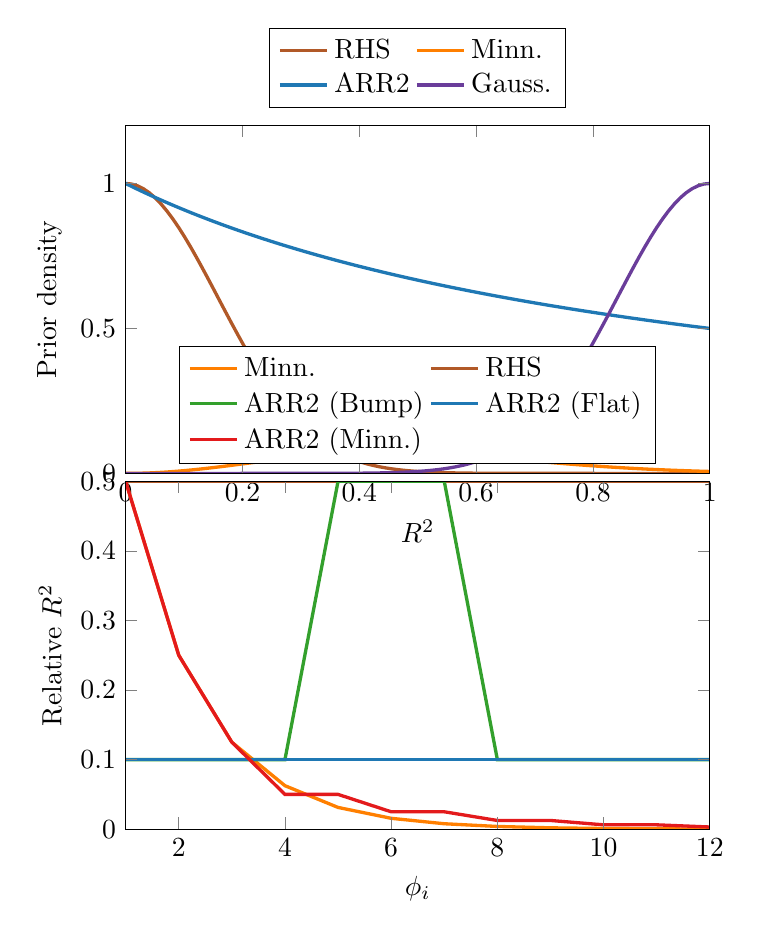
\begin{tikzpicture}
\begin{groupplot}[
    group style={
        group size=1 by 2,
        vertical sep=0.1cm,
    },
    width=9cm,
    height=6cm
]

\nextgroupplot[
    xlabel=$R^2$,
    ylabel=Prior density,
    xmin=0, xmax=1,
    ymin=0, ymax=1.2,
    domain=0:1,
    samples=100,
    axis on top,
    legend style={at={(0.5,1.05)}, anchor=south},
    legend columns=2,
    every axis legend/.append style={
        cells={anchor=west}},
    legend cell align={left},
]
\addplot[very thick, rhscolour, no markers] {exp(-x^2 / 0.05)};
\addlegendentry{RHS}
\addplot[very thick, minnesotacolour, no markers] {x^2 * exp(-x^2 / 0.2)};
\addlegendentry{Minn.}
\addplot[very thick, arr2flatcolour, no markers] {1/(1+x)};
\addlegendentry{ARR2}
\addplot[very thick, gaussiancolour, no markers] {exp(-((x-1)^2)/0.05)};
\addlegendentry{Gauss.}

\nextgroupplot[
    xlabel=$\phi_i$,
    ylabel=Relative $R^2$,
    xmin=1, xmax=12,
    ymin=0, ymax=0.5,
    ytick={0,0.1,...,0.5},
    axis on top,
    legend style={at={(0.5,1.05)}, anchor=south},
    legend columns=2,
    every axis legend/.append style={
        cells={anchor=west}},
    legend cell align={left},
]
\addplot[very thick, minnesotacolour, no markers] coordinates {(1,0.5) (2,0.25) (3,0.125) (4,0.0625) (5,0.03125) (6,0.015625) (7,0.0078125) (8,0.00390625) (9,0.001953125) (10,0.0009765625) (11,0.00048828125) (12,0.000244140625)};
\addlegendentry{Minn.}
\addplot[very thick, rhscolour, no markers] coordinates {(1,0.5) (2,0.5) (3,0.5) (4,0.5) (5,0.5) (6,0.5) (7,0.5) (8,0.5) (9,0.5) (10,0.5) (11,0.5) (12,0.5)};
\addlegendentry{RHS}
\addplot[very thick, arr2bumpcolour, no markers] coordinates {(1,0.1) (2,0.1) (3,0.1) (4,0.1) (5,0.5) (6,0.5) (7,0.5) (8,0.1) (9,0.1) (10,0.1) (11,0.1) (12,0.1)};
\addlegendentry{ARR2 (Bump)}
\addplot[very thick, arr2flatcolour, no markers] coordinates {(1,0.1) (2,0.1) (3,0.1) (4,0.1) (5,0.1) (6,0.1) (7,0.1) (8,0.1) (9,0.1) (10,0.1) (11,0.1) (12,0.1)};
\addlegendentry{ARR2 (Flat)}
\addplot[very thick, arr2minncolour, no markers] coordinates {(1,0.5) (2,0.25) (3,0.125) (4,0.05) (5,0.05) (6,0.025) (7,0.025) (8,0.0125) (9,0.0125) (10,0.00625) (11,0.00625) (12,0.003125)};
\addlegendentry{ARR2 (Minn.)}

\end{groupplot}
\end{tikzpicture}
\end{document}